\section{Caractéristiques des systèmes Big Data:}
Les méga-données sont un terme générique utilisé pour désigner toute collection de données volumineuse et complexe qui peuvent dépasser la capacité de traitement des systèmes et techniques de gestion de données conventionnels. Les applications du Big Data sont infinies. 

Les méga-données sont souvent caractérisées par le volume extrême des données, la grande variété de types de données et la vitesse à laquelle les données doivent être traitées. (Ces caractéristiques sont dites les 3V)
 
Ces caractéristiques ont été identifié pour la première fois par l'analyste Douglas Laney's membre du Gartner 10 dans un rapport publié en 2001. Plus récemment, plusieurs autres caractéristiques (autres V) ont été ajoutées aux descriptions des méga-données, notamment la véracité, la valeur et la variabilité. Bien que les méga-données ne correspondent à aucun volume de données spécifique, le terme est souvent utilisé pour décrire des téraoctets, des péta-octets et même des exa-octets de données capturées au fil du temps.

\begin{figure}[h]
	\centering
	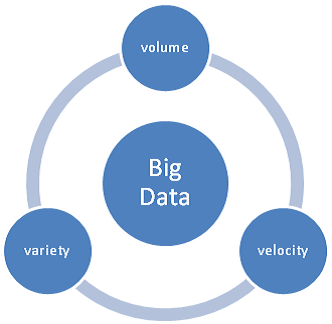
\includegraphics[scale=0.8]{img/fig3}
	\caption{Les 3 V.}
\end{figure}

Certaines personnes attribuent encore plus de V aux Big Data, les data scientiste et les consultants ont créé diverses listes contenant entre sept et 10 V.
On donne dans ce qui suit 10 caractéristiques "10V" sur les méga-données sachant que Les 3 premier critères basiques du Big Data sont le volume la vitesse ainsi que la variété :

\newcounter{compteur}
\stepcounter{compteur}
\subsection*{\arabic{compteur}. Le Volume:}
Le caractère volume est certainement celui qui est le mieux décrit par le terme Big de l'expression Big Data. Volume fait référence à la quantité d'informations, trop volumineuse pour être acquise, stockée, traitée, analysée et diffusée par des outils standards. Ce caractère peut s'interpréter comme le traitement d'objets informationnels de grande taille ou de grandes collections d'objets.

\textit{\textbf{Exemple :} les utilisateurs d'Instagram partagent 347 222 stories en 60secondes.}

\stepcounter{compteur}
\subsection*{\arabic{compteur}. La Variété:}
Elle fait référence aux différentes formes toujours croissantes que les données peuvent prendre, en effet les données Big Data ne sont pas seulement des nombres, des dates et des chaînes. Les méga-données englobent également une grande variété de types de données, y compris des données structurées dans des bases de données SQL et des entrepôts de données, des données non structurées, telles que des fichiers texte et document conservés dans des clusters Hadoop ou des systèmes NoSQL, et des données semi-structurées, telles que des journaux de serveur Web ou la diffusion des données à partir de capteurs.

\textit{\textbf{Exemple :} Un projet d'analyse des méga-données peut tenter d'évaluer le succès d'un produit et les ventes futures en corrélant les données de ventes passées, les données de retour et les données de révision des acheteurs en ligne pour ce produit.}

\stepcounter{compteur}
\subsection*{\arabic{compteur}. La vélocité:}
Dernière dimension, tout aussi importante que les précédentes, la vélocité traduit la capacité à produire rapidement les données et à les transformer en temps utile pour leurs utilisateurs. L'exercice, déjà difficile dans un contexte "classique", prend toute sa valeur lorsqu'il doit être applique à d'immenses volumes de données de toutes sortes.

\textit{\textbf{Exemple :} Google traite en moyenne plus de "40 000 requetés de recherche par seconde", ce qui représente environ 3,5 milliards de recherches par jour.}

\stepcounter{compteur}
\subsection*{\arabic{compteur}. La Véracité:}
Elle fait référence aux biais, au bruit et aux anomalies dans les données. Ou, mieux encore, il fait référence aux incertitudes et à la fiabilité des données souvent incommensurables.

\textit{\textbf{Exemple :} Dans le cadre d'un sondage réalisé par IBM, 27\% des entreprises interrogées avouent ne pas être certaines de l'exactitude des données qu'elles collectent. De même, un chef d'entreprise sur trois utilise les données pour prendre des décisions, mais n'a pas vraiment confiance. Ce manque de véracité et de qualité des données coûte environ 3,1 trillions de dollars par an aux États-Unis.}

\stepcounter{compteur}
\subsection*{\arabic{compteur}. La Valeur:}
Toutes les données collectées n'ont pas une valeur commerciale réelle et l'utilisation de données inexactes peut affaiblir les informations fournies par les applications d'analyse. Il est essentiel que les organisations utilisent des pratiques telles que le nettoyage des données et confirment que les données sont liées à des problèmes commerciaux pertinents avant de les utiliser dans un projet d'analyse de Big Data. 

On peut dire que les autres caractéristiques du Big Data n'ont pas de sens si on ne tire pas de valeur commerciale de ces données. Les Données massives offrent une valeur substantielle : comprendre mieux les clients. Les cibler en conséquence, optimiser les processus et améliorer les performances de la machine ou de l'entreprise. Avant de se lancer dans une stratégie Big Data, on doit comprendre le potentiel et les caractéristiques les plus difficiles.

\textit{\textbf{Exemple :} La mise en place d'une analyse Big Data a permis à la société de développement d'éoliennes Vestas 11 d'optimiser son processus d'identification des meilleurs emplacements pour implanter ses éoliennes. Le traitement Big Data a engendré une augmentation de la performance de production d'électricité et une réduction des coûts énergétiques associés.}

\textbf{Remarque :} Certaines personnes attribuent encore plus de V aux Big Data ; les scientifiques des données et les consultants ont créé d'autres listes en ajoutant la variabilité, la validité, la visualisation, la volatilité ainsi que la vulnérabilité.

\stepcounter{compteur}
\subsection*{\arabic{compteur}. La Variabilité:}
La variabilité dans le Big Data fait référence à plusieurs sens. Dans un premier temps elle désigne le nombre d'incohérences dans les données. Celles-ci doivent être détectées par des techniques de détection d'anomalies et de valeurs aberrantes pour faciliter la création d'analyse significative. 

Les méga-données sont également variables en raison de la diversité de dimensions résultant de multiples types et sources de données. La variabilité peut également faire référence à la vitesse incohérente à laquelle les données volumineuses sont chargées dans la base de données.

\textit{\textbf{Exemple :} L'équipe d'IBM 12 fait participer Watson 13 au célèbre jeu télévisé américain Jeopardy, un jeu ou les candidats doivent trouver les réponses à des questions posées. Watson devait "être capable de comprendre l'énoncé des questions, buzzer pour prendre la main, disséquer une réponse dans son sens pour déterminer quelle était la bonne question". Les mots n'ont pas de définitions statiques et leur signification peut varier énormément dans le contexte.}

\stepcounter{compteur}
\subsection*{\arabic{compteur}. La Validité:}
Similaire à la véracité, la validité fait référence à la précision et à la correction des données pour l'usage auquel elles sont destinées. Selon Forbes 14, environ 60\% du temps d'un scientifique est consacré au nettoyage de ses données avant de pouvoir effectuer une analyse. L'avantage de l'analyse des données massives est aussi primordial que celui des données sous-jacentes. On doit donc avoir de bonnes pratiques de gouvernance des données pour garantir une qualité des données cohérente, des définitions communes et des métadonnées.

\textit{\textbf{Exemple :} La date d'une transaction est  02/07/1994 alors que l'activité de la société a débuté en 2000.}

\stepcounter{compteur}
\subsection*{\arabic{compteur}. La Volatilité:}
On se pose les questions :\textit{‘quel âge doivent avoir les données pour qu'elles soient considérées comme non pertinentes, historiques ou obsolète ?’,  ‘Combien de temps faut-il conserver les données ?’} Avant l'ère du Big Data, en général, on stockait les données indéfiniment. Quelques téraoctets de données ne pouvaient pas engendrer de dépenses de stockage élevées. 

En raison de la vitesse et du volume de ces données massives, leur volatilité doit être soigneusement prise en compte. Il est maintenant fondamental d'établir des règles pour la disponibilité et à la mise à jour des données a de garantir une récupération rapide des informations en cas de besoin.

\textit{\textbf{Exemple :} Une entreprise e-commerce peut ne pas souhaiter conserver un historique des achats client d'un an. Parce qu'après un an la garantie par défaut sur leur produit expire, il n'y a donc aucune possibilité de restaurer ces données.}

\stepcounter{compteur}
\subsection*{\arabic{compteur}. La Visualisation:}
Une autre caractéristique du Big Data est la difficulté à les visualiser. Les logiciels de visualisation de données volumineuses actuels sont confrontés à des problèmes techniques en raison des limitations de la technologie en mémoire, de leur faible évolutivité, de leur fonctionnalité et de leur temps de réponse. Il est impossible de se fier aux graphiques traditionnels lorsqu'on essaye de tracer un milliard de points de données. Il est donc nécessaire d'avoir différentes manières de représenter des données. Telles que la mise en cluster de données ou l'utilisation de cartes d'arbres, de sunbursts, de coordonnées parallèles, de diagrammes de réseau circulaires ou de cônes. 

Si on associe cela avec la multitude de composante résultant de la variété et de la vélocité des données massives et des relations complexes qui les lient, il est possible de voir qu'il n'est pas si simple de créer une visualisation significative.

\textit{\textbf{Prenons l'exemple :} du tableau suivant qui fait apparaître deux séries de chiffres : le chiffre d'affaires en France et le chiffre d'affaires du reste du monde. La lecture de ce tableau et sa signification ne sont pas immédiates.}

\begin{figure}[h]
	\centering
	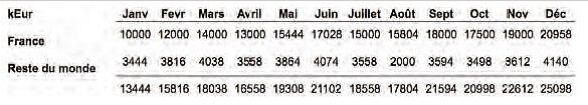
\includegraphics[scale=0.8]{img/fig5}
	\caption{Évolution du chiffre d'affaires par région.}
\end{figure}

\textit{Mais si nous représentons les séries de chiffres sous forme graphique (ci-dessous), on comprend en un coup d'œil que le chiffre d'affaires en France progresse et que le chiffre d'affaires du Reste du monde stagne.}

\begin{figure}[h]
	\centering
	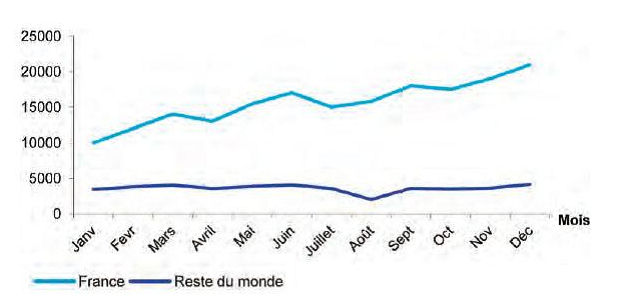
\includegraphics[scale=0.8]{img/fig6}
	\caption{Évolution du chiffre d'affaires par région.}
\end{figure}

\stepcounter{compteur}
\subsection*{\arabic{compteur}. La Vulnérabilité:}
Le Big Data apporte de nouveaux problèmes de sécurité. Malheureusement, il y a quotidiennement des violations de données massives.

\textit{\textbf{Exemple :} Rapporté par CRN15 : en mai 2016, un pirate informatique appelé Peace a posté des données sur le dark web pour les vendre, qui auraient inclus des informations sur 167 millions de comptes LinkedIn et 360 millions d'e-mails et de mots de passe pour les utilisateurs de MySpace 16.}

\begin{figure}[h]
	\centering
	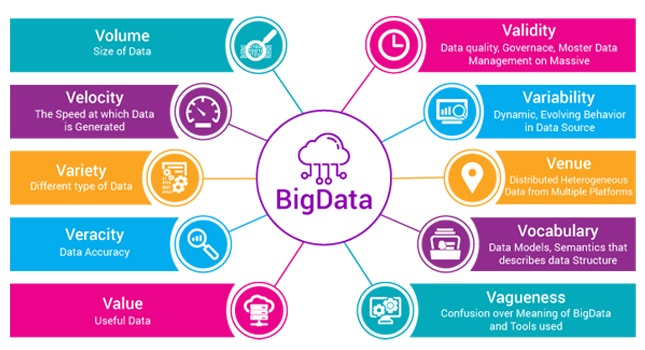
\includegraphics[scale=0.5]{img/fig4}
	\caption{Les 10 V.}
\end{figure}

\textbf{Remarque :} Il existe d'autres sources qui parlent de 54 Vs pour les caractéristiques du Big Data tel que la venue (le lieu), valence, vocabulaire, imprécision...etc.






